% !TEX root =big-fish.tex
\chapter{Collision prediction}
Movement trajectories have been designed to intersect with the goal of tolerating collisions to happen so that a collision prediction correlated to a collision avoidance algorithms can operate and add an interactive touch preventing the motion from repeating itself and making a pleasant animation that is interesting to watch.\\

Note the term prediction instead of detection; a traditional collision detection algorithm detects a collision the moment it happens, whereas what is needed is to predict collisions before they happen so that the involved fishes get enough time and space to react and avoid each other.\\

This chapter explains in details the collision prediction mechanism.

\section{Collision prevention setup}
\label{sec:setup}
The collision prediction and avoidance algorithms need to compute important parameters only once at load time to cache them for ulterior use when the animation starts which will prevent re-performing the same logic each frame and gain in terms of performance.\\

The list of operations applied to each loaded fish during the collision prevention setup includes:

\begin{itemize}

\item Add a movement listener to the fish, so that whenever its position evolves as it moves, the collision prediction algorithm gets invoked.

\item Compute trajectories intersections; will be explained in details under sub-section ~\ref{subsec:intersections}.

\item Determine which fishes are sharing the same trajectory if any. Given all trajectories are circular having the same radius and center, 2 fishes share the same trajectory if they circulate within the same plane. 2 trajectories share the same plane if they share the same relative rotated Y axis; the latter being normal to a trajectory's plane.

\item Compute the ``unit grid box'' size based on the fishes' bounding box. Briefly explained, the proximity collision prediction algorithm divides the scene in a network of big grid boxes which will be cleared and repopulated by fishes each new frame. For better performance these unit grid boxes should be big enough to fully carry the biggest fish in the scene while considering a margin. More details about calculating the unit grid box will be explained under sub-section ~\ref{subsec:ugb}.

\end{itemize}

\subsection{Intersections}
\label{subsec:intersections}

Figure~\ref{fig:intersection} lists all the data encapsulated under the Intersection structure:
\begin{figure}[H]
   \centering
   \includegraphics[scale=0.8]{figures/intersection.png}
   \caption{Intersection Data Model}
   \label{fig:intersection}
\end{figure}

In this section I will go through each field listed above.

\subsubsection{Curvilinear abscissas ($\theta_1$, $\theta_2$)}
The intersections, as opposed to what may come in mind in the first intuition, are not stored as 3D points, if they were they would need to be recalculated every time a fish avoids a collision by changing the radius of its trajectory (more details in chapter ~\ref{chap:avoidance}). To prevent this, and also because the movement is managed by $\theta_Y$ (the curvilinear abscissa of a fish within its circular trajectory), it is more efficient to define an intersection as a curvilinear abscissa as well. Proceeding thereby will make it easier to determine if a fish is close, leaving or going towards an intersection based on its curvilinear abscissa and the sign of its angular velocity $\delta _{y}$.\\

Note that an intersection has two different curvilinear abscissas $\theta_1$ and $\theta_2$ each being relative to the corresponding intersecting trajectory.\\

Another advantage of using a curvilinear abscissa to locate an intersection, is that each intersection has a diametrically opposite intersection (two intersecting trajectories always intersect twice in two diametrically opposite points), with that in mind only half intersections need to be calculated, the second half will be obtained by respectively adding $\pi$ to each of the former intersections.\\

A mathematical analysis led to the following $\theta_1$ and $\theta_2$ formulas:

\[
\left\{
\begin{array}{ll}
	\theta_2  = \arctan \left(
	\frac{\displaystyle Z_{2y} \;.\; (X_{1z} \;.\; Z_{1x} - X_{1x} \;.\; Z_{1z}) + (X_{1x} \;.\; Z_{2z} - X_{1z} \;.\; Z_{2x})}{\displaystyle Z_{1y} \;.\; (X_{1z} \;.\; X_{2x} - X_{1x} \;.\; X2_{2z})}
	\right) \\ \\
	
	\theta_1 = \pm \arccos\left(  \frac{\displaystyle Z_{2y}} {\displaystyle Z_{1y}} \;.\; \cos \theta_2 \right)
\end{array}
\right.
\]

Where $(X_{ix}, X_{iy}, X_{iz})$, and $(Z_{ix}, Z_{iy}, Z_{iz})$ are the respective coordinates of the rotated axis $\overrightarrow{X_i}$ and $\overrightarrow{Z_i}$ defining trajectory$_i$'s plane (rotated axis formulas were given in section ~\ref{subsec:swimmingstate}). Note that the sign of $\theta_1$ gets determined by processing further equations which I omitted on purpose to avoid overloading this section. It is to mention also that the equations listed above have requirements that are always verified given the trajectories design.\\

In order to visually check if the intersections were correctly calculated, a visual test has been implemented to draw the intersection of every couple of different trajectories, and check whether they are accurately located:

\begin{figure}[H]
   \centering
   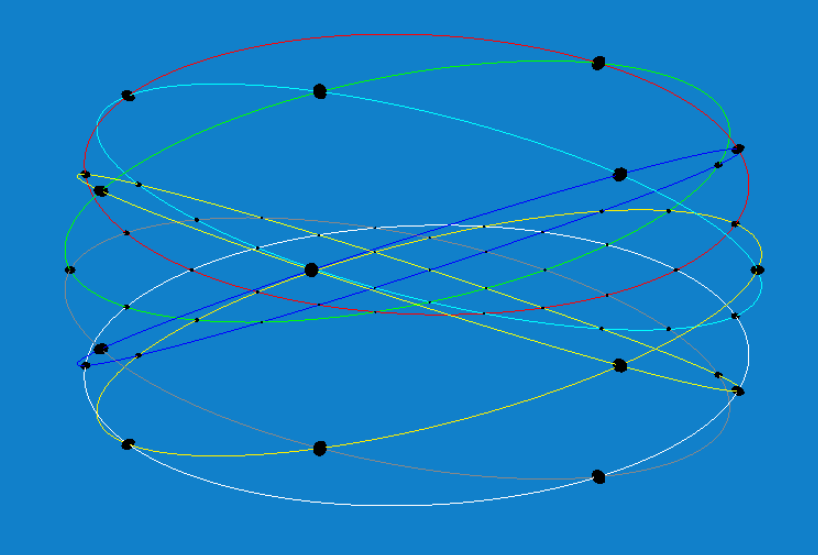
\includegraphics[scale=0.5]{figures/intersections.png}
   \caption{Intersections Test}
   \label{fig:intersections}
\end{figure}

\subsubsection{Acute angle between two trajectories ($\alpha$)}
The intersection data model also encapsulates $\alpha$ denoting the acute angle between the two planes carrying the intersecting trajectories; $\alpha$ will be used in section ~\ref{sec:dynamic.prediction}.

\begin{figure}[H]
   \centering
   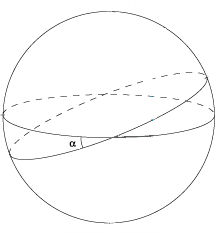
\includegraphics[scale=1]{figures/angles.jpeg}
   \caption{Angle between two trajectories ($\alpha$)}
   \label{fig:angles}
\end{figure}

If we consider $\overrightarrow{T_1}$ and $\overrightarrow{T_2}$, as two tangent vectors respectively to both trajectories passing through one of their intersections, the equation to calculate each of both vectors is as follows:\\

\[
\overrightarrow{T_i} = \left(
\begin{array}{ccc}
R \; . \; \sin \left( \theta_i + \frac{\displaystyle \pi}{2} \right) \\ \\
0 \\ \\
R \; . \; \cos \left( \theta_i + \frac{\displaystyle \pi}{2} \right)
\end{array}
\right)_{(\overrightarrow{X_i}, \overrightarrow{Y_i}, \overrightarrow{Z_i})} \; . \; CM_i
\] \\
Where $CM_i$ is the conversion matrix from trajectory$_i$'s coordinates system $(\overrightarrow{X_i}, \overrightarrow{Y_i}, \overrightarrow{Z_i})$ to the scene coordinates system $(\overrightarrow{x}, \overrightarrow{y}, \overrightarrow{z})$. $CM_i$ was explained in section ~\ref{subsec:swimmingstate}\\

$\alpha$ can be defined as  $\widehat{(\overrightarrow{T_1} \; , \; \overrightarrow{T_2})}$, which can be calculated by applying the scalar product of both vectors as follows:\\

\[
\alpha = \widehat{(\overrightarrow{T_1} \; , \; \overrightarrow{T_2})} = 
\pm \arccos \left(
\frac{\displaystyle \overrightarrow{T_1} \; . \; \overrightarrow{T_2}} {\displaystyle \| \overrightarrow{T_1} \| \; . \; \| \overrightarrow{T_2} \|} 
\right)
\] \\
Further processing is needed to determine $\alpha$'s sign, but will be omitted to alleviate this section.

\subsubsection{Reference to the intersecting fish}

The avoidance state loops through the avoiding fish close intersections to predict whether returning to the previous trajectory would result in a collision. The prediction requires access to parameters such as the bounding box of the intersecting fishes, as well as their trajectories and velocities. These parameters are encapsulated under the fish structure, which justifies the need to reference the intersecting fish from an intersection.


\subsubsection{Intersections modeled as circular bidirectional linked list nodes }
For better performance, the avoidance algorithm needs to efficiently loop over neighbor intersections in both directions (clockwise and counter colockwise) given a close intersection. A bidirectional circular linked list has been adopted for this purpose. Figure~\ref{fig:linkedlist} gives a preview of the relationships between intersections:

\begin{figure}[H]
   \centering
   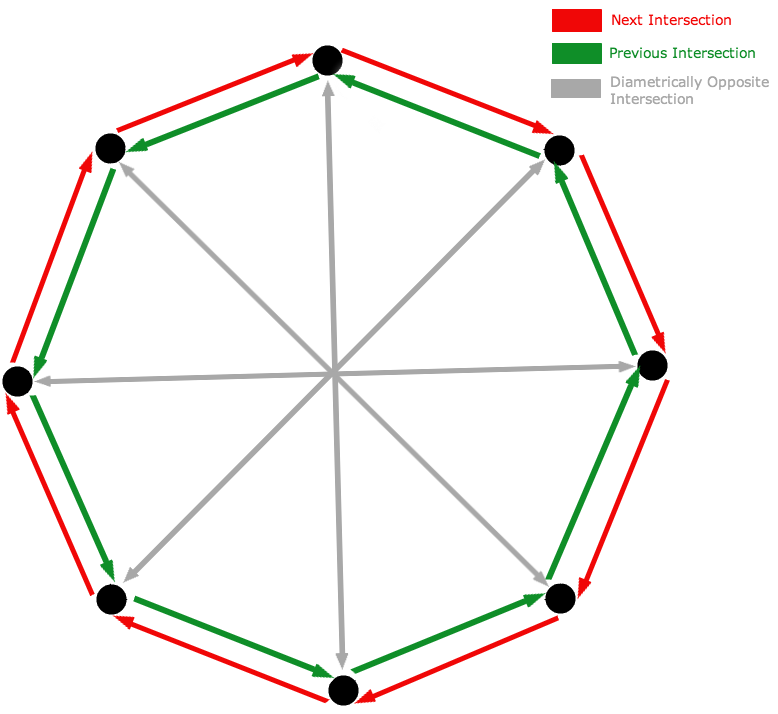
\includegraphics[scale=0.58]{figures/linkedlist.png}
   \caption{Intersections circular bidirectional linked list}
   \label{fig:linkedlist}
\end{figure}

\subsubsection{Mapping fishes to intersections}
The proximity collision prediction algorithm (section~\ref{sec:static.prediction}) forwards a couple of fishes to the kinetics based prediction algorithm (section~\ref{sec:dynamic.prediction}) whenever they are close enough. The latter algorithm needs an efficient access to the appropriate intersection given a couple fishes. This need can be fulfilled by encapsulating an associative array under the fish structure that maps each intersecting fish's id to the corresponding intersection.\\

Note that each couple of different trajectories intersect twice in two diametrically opposite points, meaning mapping a fish's id to only one intersection is not enough, which explains the need to reference the diametrically opposite intersection in the intersection structure (see figures~\ref{fig:intersection} and ~\ref{fig:linkedlist}).

\subsection{Unit grid box}
\label{subsec:ugb}

The proximity collision prediction algorithm divides the scene into a network of big grid boxes, which for better performance (see section~\ref{subsec:performancerec}) should be big enough to carry any fish in the scene while considering a margin. However since the orientation of a fish keeps changing as it moves, the corresponding bounding box edges adapt by changing accordingly. Given no edge can surpass the initial bounding box diameter no matter the orientation, the biggest diameter of all fishes' bounding boxes plus a margin has been adopted as the edge of the unit grid box. The purpose of the margin will be explained under section~\ref{sec:static.prediction}.\\

Note that by the time this document was written, ThreeJS being a new framework, offered only a utility method to calculate a static bounding box of a raw morph regardless of its position, scale or Euler rotations (orientation). Support for those was implemented from scratch.

\subsection{Avoidance trajectories margin}
\label{subsec:avoidance-margin}

When a fish avoids a collision it switches the radius of its trajectory to a smaller one. The difference between the two radiuses ($\Delta_{R}$) needs to be calculated in a way that guarantees fishes swimming within a sphere surface having $R$ as radius, will never collide with fishes swimming within a smaller sphere surface having $(R-\Delta_{R})$ as radius (more details on this through chapter~\ref{chap:avoidance}). For this reason $\Delta_{R}$ needs to match half the sum of the two biggest fishes' thicknesses in the scene. Given a fish's orientation is directed by its relative Z axis, the thickness of a fish cannot exceed the maximum of its bounding box's Y and X edges. Note that the margin treated in this section is different from the margin mentioned in the previous section (~\ref{subsec:ugb}).

\section{Proximity collision prediction}
\label{sec:static.prediction}

The proximity collision prediction is the first layer of the prediction algorithm, it filters fishes that are good candidates for imminent collisions and forwards them to the kinetics based algorithm for further processing. The main purpose of using the proximity prediction is to minimize invoking the kinetics based algorithm as possible given its complexity (see section~\ref{sec:dynamic.prediction}).\\

If we consider a three dimensional grid of big boxes serving as a large scaled coordinate system, the idea is to perform the following operations whenever a movement listener gets notified by a change of a fish's location:
\begin{itemize}

\item Calculate the bounding box of the fish, considering the new position, the scale, and Euler rotations.

\item Add margins to the new bounding box volume. The margins serve as the security distance that separates two fishes, lower than which the kinetics based prediction algorithm gets invoked.

\item Convert the position and dimensions of the bounding box to the large scaled coordinate system; let's denote the result ``normalized bounding box"; given the large scaled coordinate system unit is big enough to carry the biggest fish in the scene with a margin, the normalized bounding box volume will never exceed a maximum of 8 unit boxes (i.e. when a fish overlaps a corner of a normalized unit box which implies overlapping the 8 normalized unit boxes sharing that corner), but can be a minimum of only one unit box. A performance test has been recorded in this regard (see section ~\ref{subsec:performancerec}).

\item Use an associative array to determine which fishes are sharing unit boxes as follows:

\begin{itemize}

\item Convert each unit box coordinates to a string key.

\item Check if the key is already mapping to previously processed fishes. If so a grid box population event gets fired, thereby triggering the kinetics based prediction algorithm. Otherwise a new entry gets added to the associative array. 

\item Each new frame the associative array gets cleared, and re-populated from scratch.

\end{itemize}
\end{itemize}

This logic will prevent applying the kinetics based prediction algorithm on fairly distant fishes. Each fish will just need to check for collisions only with fishes that share one or more of its populated unit boxes.\\

Note that a caching mechanism has been placed to prevent checking collisions multiple times for couples of fishes sharing more than one unit box.\\

\subsection{Performance}
\label{subsec:performancerec}

A test has been run for a duration of 5 minutes with 11 fishes in the scene to record some key performance indicators and prove the efficiency of the proximity collision prediction algorithm compared to simply using a nested loop.

\subsubsection{First record}

Table ~\ref{tab:numberfishesunitbox} presents records of how often in average a unit box gets populated by a number of fishes.

\begin{table}[H]
\centering
\begin{tabular} { | l | l | }
\hline
\textbf{Number of fishes per unit box} & \textbf{Frequency (\%)} \\
\hline
1 & 85.74 \\
\hline
2 & 13.21 \\
\hline
3 & 0.91 \\
\hline
4 & 0.09 \\
\hline
5 & 0.044 \\
\hline
\end{tabular}
\caption{Performance - Number of fishes per normalized unit box}
\label{tab:numberfishesunitbox}
\end{table}

Given the first fish that populates a unit box never checks for collisions, we obtain in average $(1 \times 0.13 + 2 \times 0.0091 + 3 \times 0.0009 + 4 \times 0.00044) \approx$ \textbf{0.155}  collision verification per unit box per frame.

\subsubsection{Second record}

Depending on its position, size and rotations, a fish may populate 1 to 8 normalized unit boxes. Table ~\ref{tab:numberunitboxfish} presents how often in average a fish populates a number of unit boxes.

\begin{table}[H]
\centering
\begin{tabular} { | l | l | }
\hline
\textbf{Number of unit boxes populated by a fish} & \textbf{Frequency (\%)} \\
\hline
1 & 29.6 \\
\hline
2 & 47.85 \\
\hline
4 & 20.08 \\
\hline
8 & 2.46 \\
\hline
\end{tabular}
\caption{Performance - Number of normalized unit boxes populated by a fish}
\label{tab:numberunitboxfish}
\end{table}

Which gives an average of $(1 \times 0.296 + 2 \times 0.4785 + 4 \times 0.2008 + 8 \times 0.0246) \approx$ \textbf{2.253} unit boxes populated per fish per frame.

\subsubsection{Conclusion}

Each frame, one fish populates 2.253 unit boxes, from which only 15.5\% trigger collision verifications. Given the test was run with 11 fishes in the scene, we obtain in average $(11 \times 2.253 \times 0.155) \approx $ \textbf{3.84} collision verifications per frame, compared to $(\sum\limits_{i=2}^{11} i) =$ \textbf{65} collision verification if a nested loop checking for every couple fishes has been adopted.

\subsection{Appropriate states for avoidance}
When a fish avoids a collision, it reduces the radius of its circular trajectory leaving enough margin to prevent any overlapping. However in order to keep the movement look natural, the avoiding fish has to follow a link trajectory towards the smaller radius trajectory. A fish's state is appropriate for avoidance when it's either in the swimming state, or in the avoiding state but not in a link trajectory (see chapter~\ref{chap:avoidance} for more details).\\

The states Dying, Reviving, Dead, and Resizing are not appropriate for avoidance. When a fish is in one of these states (which is very rare) collisions may happen.\\

When a fish's state is not appropriate for avoidance it won't be placed in the grid, and thus won't be considered by any of both collision prediction algorithms.

\label{subsec:appropriatestate}


\section{Collision prediction based on kinetics}
\label{sec:dynamic.prediction}

The algorithm in this section predicts accurately whether a couple of close fishes are willing to collide based on kinetics. In order to simplify things, a couple of intersecting trajectories' arcs get projected into a 2D plane. The projection doesn't perfectly match the motion in 3D, but approximates accurately enough to predict any collision before it happens with a comfortable time and space margin. Figure~\ref{fig:projection-abcd} illustrates the projection:

\begin{figure}[H]
   \centering
   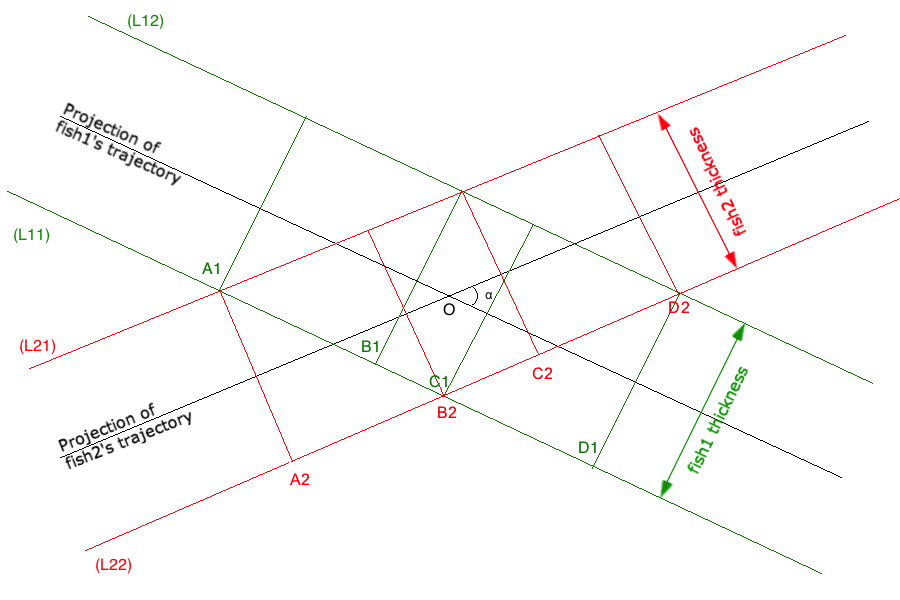
\includegraphics[scale=0.5]{figures/projection-abcd.png}
   \caption{2D projection - same key positions order for both fishes}
   \label{fig:projection-abcd}
\end{figure}

\begin{itemize}
\item Given that a fish's orientation is directed by its relative Z axis, the \uline{thickness} of a fish cannot exceed the maximum of its bounding box's Y and X edges.
\item $\alpha$ is the angle between the two planes carrying both trajectories (see sub-section ~\ref{subsec:intersections}).
\item $(L_{ij})$ represent the borders delimiting the area within which fish$_i$ is swimming.
\item $A_i, B_i, C_i$ and $D_i$ are key locations for the kinetics based algorithm (see section~\ref{subsec:kinetics}). They can be defined as follows:
\begin{itemize}
\item $A_i = (L_{i1}) \cap (L_{\overline{i}1})$, with $\overline{i} = 2 $ if (i = 1), otherwise $\overline{i} = 1$.
\item $B_i = (L_{i2}) \cap (L_{\overline{i}1})$.
\item $C_i = (L_{i1}) \cap (L_{\overline{i}2})$.
\item $D_i = (L_{i2}) \cap (L_{\overline{i}2})$.
\end{itemize}
 
\end{itemize}

Note that in the definitions above, the key locations have been defined as points; later on, they should be thought of as the orthogonal lines to the borders passing through these points. That said, if through what follows the notation $A_iB_i$ for instance gets used, it should be thought of as the distance between two parallel lines rather than two points. These lines will be located by their curvilinear abscissas within their corresponding trajectories.\\

Note also that in figure~\ref{fig:projection-abcd} the order of the key positions is the same for both fishes, however when their thicknesses' difference is big enough, the order changes. Figure~\ref{fig:projection-acbd} shows that for fish$_1$ (less thick) the key positions order is A$_1$, B$_1$, C$_1$ then D$_1$, whereas for fish$_2$ (thicker) the order is A$_2$, C$_2$, B$_2$ then D$_2$.
\begin{figure}[H]
   \centering
   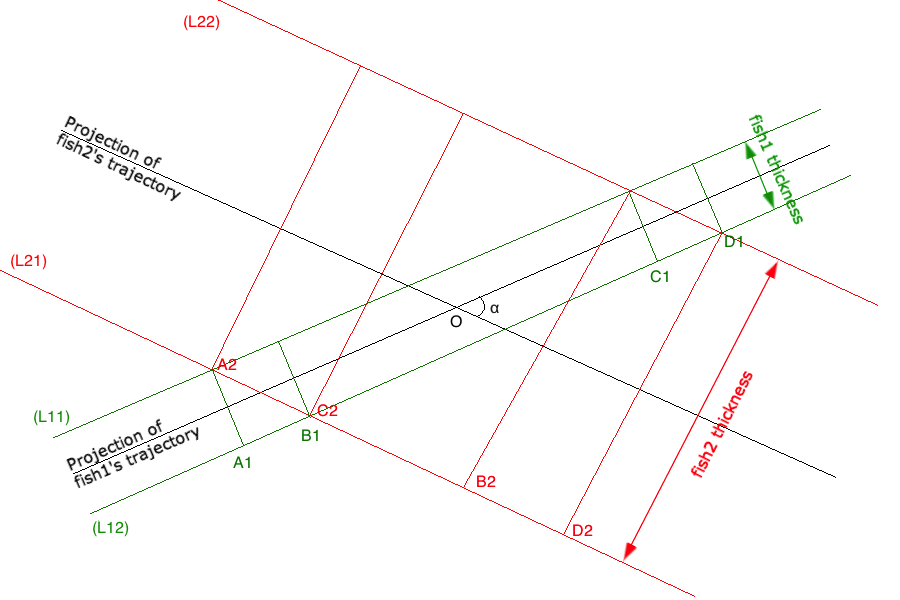
\includegraphics[scale=0.5]{figures/projection-acbd.png}
   \caption{2D projection - different key positions order per fish}
   \label{fig:projection-acbd}
\end{figure}

The key locations order is important when a fish is trying to return from an avoidance trajectory, and predicting whether its return would result in a collision (more details in chapter~\ref{chap:avoidance}).

\subsection{Locating the key positions}

Following are the mathematical formulas required to compute the key locations:\\

\begin{gather*}
A_iB_i = \abs{\frac{thickness_i}{\tan(\alpha)}} \;\;\;,\;\;\; A_iC_i = \abs{\frac{thickness_{\overline{i}}}{\sin(\alpha)}} \;\;\; , \;\;\; A_iD_i = A_iB_i + A_iC_i \\\\
OA_i = \frac{A_iD_i}{2} \;\;\; , \;\;\; OB_i = \abs{OA_i - A_iB_i} \;\;\; , \;\;\; \overline{OD_i} = -\overline{OA_i} \;\;\; , \;\;\; \overline{OC_i} = -\overline{OB_i} 
\end{gather*}

\begin{gather*}
sign(\overline{OA_i}) = sign(\delta_i); where\: \delta_i = (\theta_{Y_i} - \theta_i) [2\pi]; with \: \delta_i \in ]-\pi, \pi]\\\\
sign(\overline{OB_i}) = sign(\overline{OA_i}) \times sign(OA_i - A_iB_i)
\end{gather*}

Note that $\theta_{Y_i}$ is the curvilinear abscissa of fish$_i$ within its trajectory, while $\theta_i$ is the curvilinear abscissa of the intersection O relatively to fish$_i$'s trajectory. All $\theta_i$'s have been calculated and cached during the collision prevention setup. That said, the curvilinear abscissas for the key positions relatively to the corresponding trajectory can be obtained as follows:
\[
\theta_{A_i} = \frac{\overline{OA_i}}{R} + \theta_{Y_i} \;\;\; , \;\;\; \theta_{B_i} = \frac{\overline{OB_i}}{R} + \theta_{Y_i} \;\;\; , \;\;\; \theta_{C_i} = \frac{\overline{OC_i}}{R} + \theta_{Y_i} \;\;\; , \;\;\; \theta_{D_i} = \frac{\overline{OD_i}}{R} + \theta_{Y_i}
\]
Where R denotes the radius of the circular trajectory.

\subsection{Applying kinetics to the two dimensional projection}
\label{subsec:kinetics}

Based on the 2D projection, the logic applied to predict a collision, depends on many scenarios. Figure~\ref{fig:prediction-scenarios} illustrates all the possible scenarios:

\begin{figure}[H]
   \centering
   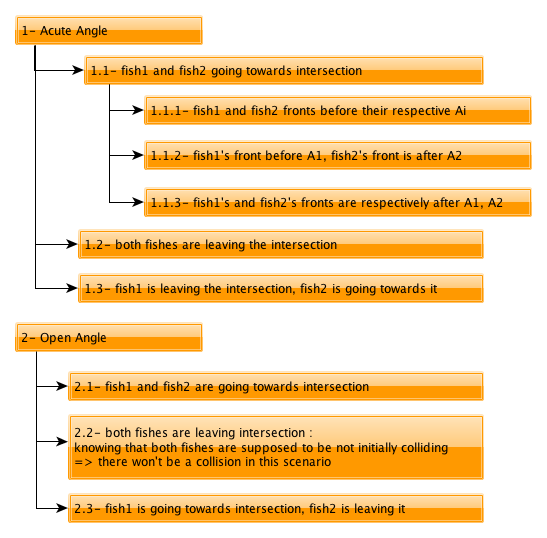
\includegraphics[scale=0.75]{figures/prediction-scenarios.png}
   \caption{Collision prediction scenarios}
   \label{fig:prediction-scenarios}
\end{figure}

Where the angle being considered as acute or open refers to $\widehat{A_1 O A_2}$, which is either $\alpha$ or $(\pi - \alpha)$ depending on the fishes positions. Note that $\alpha$ is the angle between both planes carrying the trajectories, it was calculated and cached during the collision prevention setup.\\

The rest of this section will go through the first case 1.1.1, which should be sufficient to inspire processing the rest of the cases. Figure~\ref{fig:case111} presents case 1.1.1:\\

\begin{figure}[H]
   \centering
   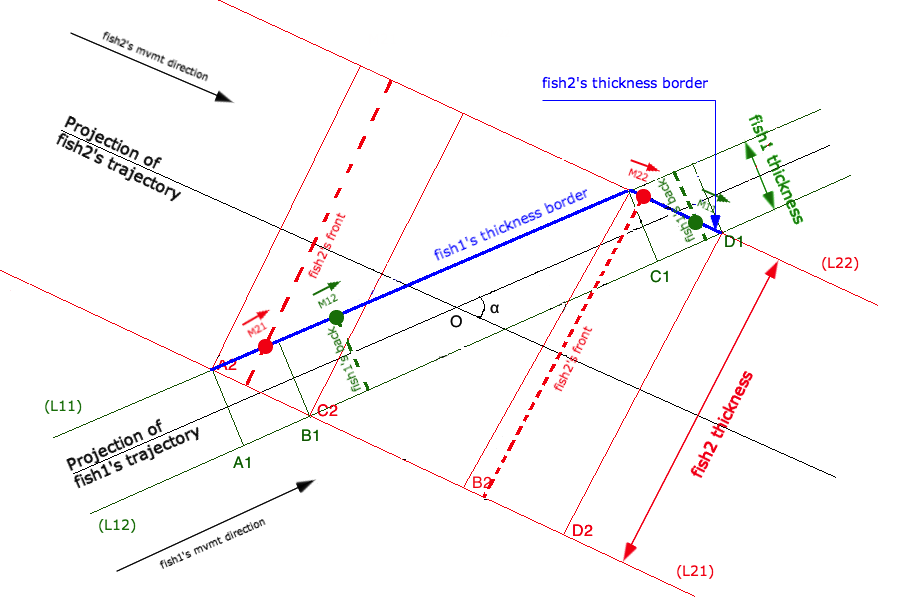
\includegraphics[scale=0.5]{figures/case111.png}
   \caption{Acute angle, both fishes going towards intersection, both fishes fronts are before A$_1$, A$_2$}
   \label{fig:case111}
\end{figure}

The critical area for each fish is delimited by A$_i$ and D$_i$, meaning a collision between both is possible (but not certain) only when both are inside their critical areas. The required steps to accurately predict a collision are the following:

\subsubsection{First step}
Determine which fish will reach A$_i$ first. Note that for better accuracy in the estimations, the fish's front position will be considered instead of simply its position. If we consider T$_1$ and T$_2$ as the necessary durations for fish$_1$ and fish$_2$ to arrive respectively to A$_1$, A$_2$, the fish arriving in a minimum duration will be the first. T$_1$ and T$_2$ can be calculated as follows:
\begin{gather*}
T_1 = \frac{\abs{\theta_{F1} - \theta_{A1}}}{\abs{\delta_{Y1}}} \;\;\;,\;\;\; T_2 = \frac{\abs{\theta_{F2} - \theta_{A2}}}{\abs{\delta_{Y2}}} 
\end{gather*}
Where $\theta_{Fi}$ is the curvilinear abscissa of the corresponding fish's front, $\theta_{Ai}$ is the curvilinear abscissa of $A_i$ and $\delta_{Yi}$ denoting the angular velocity. Let's call fish$_1$ the fish that will arrive first.

\subsubsection{Second step}
Guarantee that fish$_1$'s back will also arrive to A$_1$ before fish$_2$'s front reaches A$_2$. This could be investigated by applying the same logic described above.

\subsubsection{Third step}
Guarantee that fish$_1$'s back will keep its position in front of fish$_2$'s front, all along the critical area, otherwise a collision may happen. Notice that from A$_1$ to C$_1$ for fish$_1$ (A$_2$ to B$_2$ for fish$_2$) if a collision would happen, the first contact point would be located within fish$_1$'s thickness border (the blue highlighted line), whereas from C$_1$ to D$_1$ for fish$_1$ (B$_2$ to D$_2$ for fish$_2$) the first contact point would be located within fish$_2$'s thickness border. In other words, if we define the following mobile points:

\begin{itemize}
\item $M_{12} = (fish1's\; back) \cap (L_{11})$; where $M_{12} \in [A_1C_1]$.
\item $M_{21} = (fish2's\; front) \cap (L_{11})$; where $M_{21}  \in [A_2B_2]$.
\item $M_{11} = (fish1's\; back) \cap (L_{22})$; where $M_{11}  \in [C_1D_1]$.
\item $M_{22} = (fish2's\; front) \cap (L_{22})$; where $M_{22}  \in [B_2D_2]$.
\end{itemize}

It is obvious to notice that while M$_{12}$ has the same speed as fish$_1$, M$_{11}$ is faster since fish2's thickness border (highlighted in blue) is longer than $C_1D_1$. Following the same logic for fish$_2$, M$_{21}$ is also faster than M$_{22}$. With that in mind, it is important to assert two facts to ensure a collision won't happen within the critical area:

\begin{itemize}
\item First guarantee that M$_{21}$ won't catch M$_{12}$ all along fish1's thickness border. This could be investigated by checking which of both fishes will arrive first to C$_1$, respectively B$_2$.
\item Second guarantee that M$_{22}$ won't catch M$_{11}$ all along fish2's thickness border. This could be investigated by checking which of both fishes will arrive first to D$_i$.
\end{itemize}

The same logic used in the first step can be applied here to investigate both of the above propositions.

\newpage